\documentclass[11pt]{report}
\usepackage{textcomp}

\usepackage{titlesec}
\titlespacing*{\section}
{0pt}{\baselineskip}{0em}
\titlespacing*{\subsection}
{0pt}{\baselineskip}{0em}

\usepackage{geometry}
\geometry{left=1in, right=1in, top=1in, textheight=9in}

\usepackage{enumitem}
\newlist{steps}{enumerate}{1}
\setlist[steps, 1]{wide=0pt, leftmargin=\parindent, label=Step \arabic*:}

\usepackage{fancyhdr}
\fancypagestyle{plain}{%
    \fancyhf{} % clear all header and footer fields
    \fancyfoot[C]{\sffamily\fontsize{.75em}{.75em}\selectfont\thepage} % except the center
    \renewcommand{\headrulewidth}{0pt}
    \renewcommand{\footrulewidth}{0pt}
}
\pagestyle{plain}

\usepackage{graphicx}
\graphicspath{ {./media/} }

\usepackage{minted}
\usepackage{xcolor}
\definecolor{LightGray}{gray}{0.9}

\usepackage{setspace}
\doublespacing

% make fancy title page
\makeatletter
\newcommand{\@labsection}{000}
\newcommand{\labsection}[1]{
    \renewcommand{\@labsection}{#1}
}

\newcommand{\@labnumber}{0}
\newcommand{\labnumber}[1]{
    \renewcommand{\@labnumber}{#1}
}

\newcommand{\@shortsubmitted}{1/1/70}
\newcommand{\shortsubmitted}[1]{
    \renewcommand{\@shortsubmitted}{#1}
}

\lfoot{\footnotesize \textit{University of Arkansas \\ EECS Department}}
\rfoot{\footnotesize \textsl{\@shortsubmitted}}

\renewcommand{\maketitle}{
    \newgeometry{left=1in, right=1in, top=1.75in, textheight=8.25in}
    \singlespacing
    \begin{center}
        {\huge \bf CSCE 22104} \\
        \vspace{2.5em}
        {\Large \bf Lab Report} \\
        \vspace{2em}
        \noindent\rule{20em}{0.4pt} \\
        \vspace{1em}
        {\Large \@author} \\
        \vspace{.75em}
        {\normalsize ID: 011019116} \\
        \vspace{.75em}
        {\normalsize Lab Section \@labsection} \\
        \vspace{.75em}
        {\normalsize Lab \@labnumber} \\
    \end{center}
    \newpage
    \restoregeometry
}

\makeatother


% TEXTWIDTH = 100
\begin{document}
\title{Lab Report 11}
\author{Brent Marcus Orlina}

\labsection{001}
\labnumber{11}

\shortsubmitted{4/30/25}

\maketitle

\section*{Introduction}
The goal of this lab was to integrate instruction memory, which is a memory component that holds the
instructions that the CPU should execute. The previously provided memory component only held 16
bytes, or eight 16-bit instructions. However, the CPU supports fifteen instructions so the memory
component was updated to hold up to 32 bytes, or sixteen 16-bit instructions. The instruction memory
should also read from a text file called \verb|instr.txt| instead of \verb|in.txt|, which the
previously integrated memory, the data memory, read in from.

Another component that is provided is the program counter register, \verb|PC_REG|. The purpose of
this component is to hold the address that the CPU should read from in the instruction memory. After
each clock cycle, the program counter should increment by two to read the next instruction since
each instruction is two bytes long. The program counter should also reset to 0 if the CPU has its
input port \verb|clear| as 0, since it is active low.

\section*{Approach}
\begin{listing}[h!]
    \inputminted[
        frame=lines,
        breaklines,
        linenos,
        tabsize=4,
        fontsize=\footnotesize,
        bgcolor=LightGray
    ]{vhdl}{./media/Memory-generics.vhd}
    \caption{The memory component's new generic.}
    \label{listing:memory-generics}
\end{listing}

\begin{listing}[h!]
    \inputminted[
        frame=lines,
        breaklines,
        linenos,
        tabsize=4,
        fontsize=\footnotesize,
        bgcolor=LightGray
    ]{vhdl}{./media/Memory-signals.vhd}
    \caption{The memory component's new signal.}
    \label{listing:memory-signals}
\end{listing}

Listing \ref{listing:memory-generics} shows the generics that the memory component now uses. The
\verb|INPUT| generic of the memory component, the data that the component is intialized to, is now
\verb|instr.txt| by default. This means that even the data memory reads in \verb|instr.txt|, filling
the it with "random" junk data. This is done because there was trouble with changing the
\verb|INPUT| generic from the default by using a generic map, thus the default had to be changed and
its effect of filling the data memory with junk data is considered worth it since it has minimal
impact.

Listing \ref{listing:memory-signals} shows the type \verb|mem_type| changed from an array of 16
bytes to an array of 32 bytes. This is so that all of the instructions supported by the CPU can be
tested since there are 15 total instructions with each instruction having a length of two bytes,
thus all 15 instructions can fit into memory.

\begin{listing}[h!]
    \inputminted[
        frame=lines,
        breaklines,
        linenos,
        tabsize=4,
        fontsize=\footnotesize,
        bgcolor=LightGray
    ]{vhdl}{./media/PC_REG-ports.vhd}
    \caption{The program counter register's ports.}
    \label{listing:PC_REG-ports}
\end{listing}

Listing \ref{listing:PC_REG-ports} shows the ports of the provided program counter register
component. Since the program counter increments after each clock cycle, it is synchronous and thus
needs a \verb|clk| input port. It also resets back to 0 if the CPU clears so it also takes an input
port \verb|reset|. The ports \verb|Input| and \verb|Output| are for the program counter, which feeds
back to itself. 

\begin{listing}[h!]
    \inputminted[
        frame=lines,
        breaklines,
        linenos,
        tabsize=4,
        fontsize=\footnotesize,
        bgcolor=LightGray
    ]{vhdl}{./media/PC_REG-implementation.vhd}
    \caption{The program counter register's implementation.}
    \label{listing:PC_REG-implementation}
\end{listing}

Listing \ref{listing:PC_REG-implementation} shows the implementation of the provided program counter
register. It uses two signals \verb|Reg| and \verb|Delay|. The signal \verb|Reg| is simply connected
to the output port \verb|Output|. A signal for this is needed since VHDL does not allow an output
port to be set using itself.

Since the register is synchronous to the clock, the main process is sensitive to the input port
\verb|clk|. However, the reset is asynchronous, so the main process is also sensitive to the input
port \verb|reset|. Firstly, it checks if the reset signal is inactive to reset the register back to
0 since the CPU uses active low for its reset signal. If there is a signal to reset, it resets the
register to 0 and activates the \verb|Delay| signal.

If there is no signal to reset, it checks whether \verb|clk| is in a rising edge since it is
synchronous to the clock. During a rising edge, it checks whether there is a delay signal, through
the signal \verb|Delay|. This is so that in the clock cycle right after a reset signal is made, the
register will output a $0$. If there is no delay signal, the register would immediately increment
the register in the following clock cycle of the delay signal, and thus the program counter wouldn't
really start at $0$. This can be seen when the \verb|Delay| signal is \verb|'1'|. It sets \verb|Reg|
to 0 and deactivates the delay signal so that the program counter can be incremented in the next
clock cycle.

\begin{listing}[h!]
    \inputminted[
        frame=lines,
        breaklines,
        linenos,
        tabsize=4,
        fontsize=\footnotesize,
        bgcolor=LightGray
    ]{vhdl}{./media/CPU-ports.vhd}
    \caption{The CPU component's ports.}
    \label{listing:CPU-ports}
\end{listing}

Listing \ref{listing:CPU-ports} shows the CPU-components ports. Since the instructions are now being
fetched from memory, there is no reason for the CPU to have an input port that receives instructions
and thus the \verb|instruction| input port is removed.

\newpage

\begin{listing}[h!]
    \inputminted[
        frame=lines,
        breaklines,
        linenos,
        tabsize=4,
        fontsize=\footnotesize,
        bgcolor=LightGray
    ]{vhdl}{./media/CPU-components_signals.vhd}
    \caption{The other components and signals that the CPU component uses.}
    \label{listing:CPU-components_signals}
\end{listing}

Listing \ref{listing:CPU-components_signals} shows the components and signals that the CPU uses. The
CPU of course uses the new program counter register component \verb|PC_REG|. The new signal
\verb|PC| is used as the program counter, which is the address that the instruction memory reads
from to output the current instruction to the new signal \verb|Instruction|.

\newpage

\begin{listing}[h!]
    \inputminted[
        frame=lines,
        breaklines,
        linenos,
        tabsize=4,
        fontsize=\footnotesize,
        bgcolor=LightGray
    ]{vhdl}{./media/CPU-fetch.vhd}
    \caption{The instruction fetch phase of the CPU implementation.}
    \label{listing:CPU-fetch}
\end{listing}

Listing \ref{listing:CPU-fetch} shows the instruction fetch phase of the CPU. A \verb|PC_REG|
component is initialized. Notably, the signal \verb|PC| is connected to both the \verb|Input| and
\verb|Output| ports of the PC register component. This is because the \verb|PC| signal is being
incremented within the \verb|PC_REG| component after a clock cycle and the result should be
outputted to the \verb|PC| signal again.

The \verb|InstructionMemory| component is initialized. Notably, the ports \verb|read_en| and
\verb|write_en| are constantly active and inactive respectively since the CPU instructions should
only be read and never be modified. Of course this is not how it works in the real world. However in
this simulation, there is no reason for the instructions to change. The port \verb|addr| is mapped
to \verb|PC| since the CPU should read the next instruction in memory after every clock cycle. Since
this memory component will never be written to, the \verb|data_in| port is set to a constant of $0$.
The data read is outputted to the signal \verb|Instruction|, which is split to its respective
sections \verb|OP|, \verb|RD|, \verb|RS|, and \verb|RT| on lines 23 to 25.

\section*{Experimentation}
The integration of the new instruction memory component was tested by writing a testbench for the
CPU component that simply runs the clock for however long is needed to test all the given
instructions. Along with the testbench, the \verb|instr.txt| file is given which contains all of the
given instructions to be tested, used to intialize the instruction and data memories.

\section*{Results \& Discussion}
\begin{figure}[h!]
    \centering
    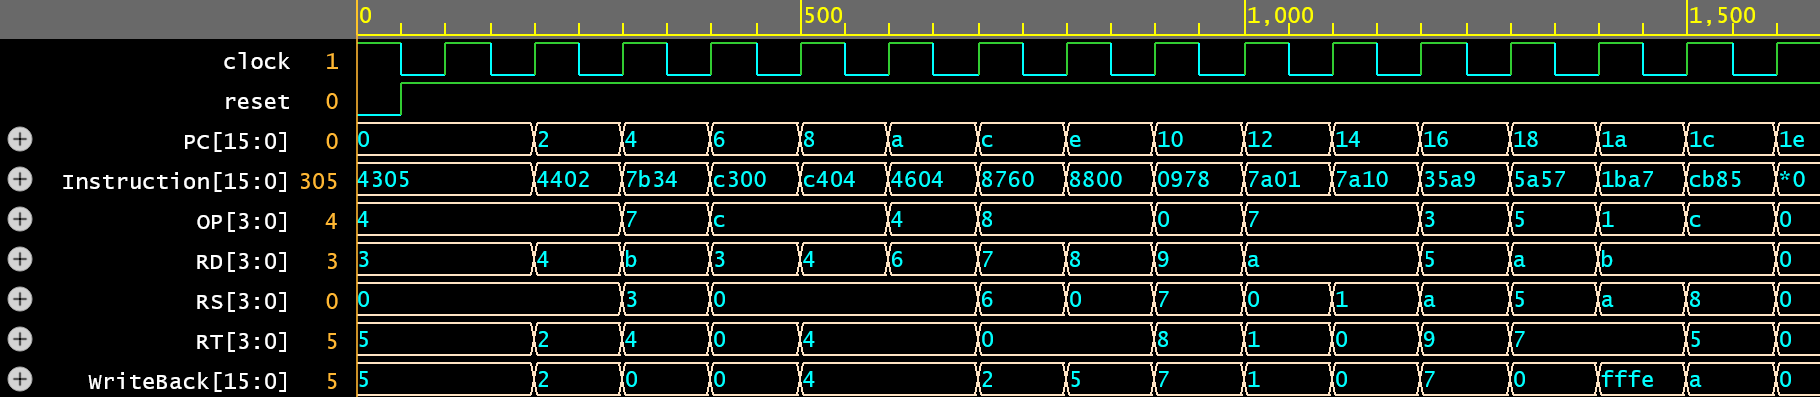
\includegraphics[width=0.95\textwidth]{CPU-waveform_hex}
    \caption{The waveform for the CPU component with a radix of hex.}
    \label{fig:CPU-waveform_hex}
\end{figure}

\begin{figure}[h!]
    \centering
    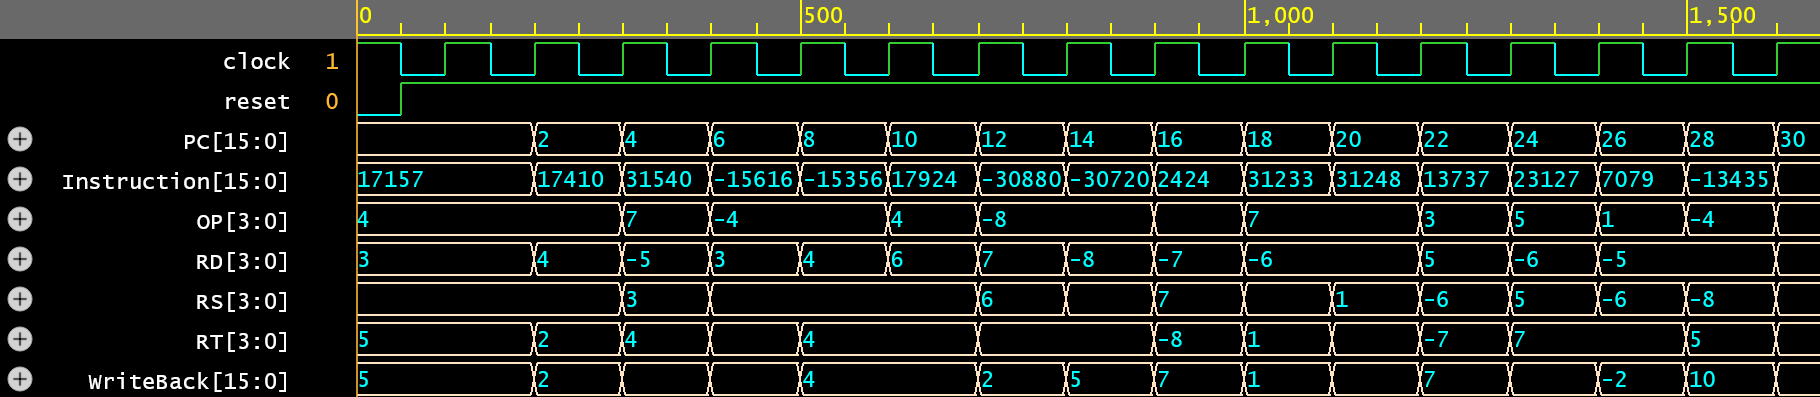
\includegraphics[width=0.95\textwidth]{CPU-waveform_signed}
    \caption{The waveform for the CPU component with a radix of signed decimal.}
    \label{fig:CPU-waveform_signed}
\end{figure}

\begin{table}[ht!]
    \centering
    \begin{tabular}{|l||c|c|c|c|c|} 
     \hline
     Instruction & op & rd & rs & rt & value (of rd) \\
     \hline
     \verb|ADDI  R3,  R0,  5| & \verb|0x4| & \verb|0x3| & \verb|0x0| & \verb|0x5| & \verb| 5| \\ 
     \hline                                                                                
     \verb|ADDI  R4,  R0,  2| & \verb|0x4| & \verb|0x4| & \verb|0x0| & \verb|0x2| & \verb| 2| \\
     \hline                                                                              
     %
     \verb|SLT  R11,  R3, R4| & \verb|0x7| & \verb|0xB| & \verb|0x3| & \verb|0x4| & \verb| 0| \\
     \hline                                                                              
     %
     \verb|SW    R3,   0(R0)| & \verb|0xC| & \verb|0x3| & \verb|0x0| & \verb|0x0| & \verb| 0| \\
     \hline                                                                                
     \verb|SW    R4,   4(R0)| & \verb|0xC| & \verb|0x4| & \verb|0x0| & \verb|0x4| & \verb| 4| \\ 
     \hline                                                                                
     %
     \verb|ADDI  R6,  R0,  4| & \verb|0x4| & \verb|0x6| & \verb|0x0| & \verb|0x4| & \verb| 4| \\
     \hline                                                                                
     %
     \verb|LW    R7,   0(R6)| & \verb|0x8| & \verb|0x7| & \verb|0x6| & \verb|0x0| & \verb| 2| \\
     \hline                                                                                
     \verb|LW    R8,   0(R0)| & \verb|0x8| & \verb|0x8| & \verb|0x0| & \verb|0x0| & \verb| 5| \\
     \hline
     %              
     \verb|ADD   R9,  R7, R8| & \verb|0x0| & \verb|0x9| & \verb|0x7| & \verb|0x8| & \verb| 7| \\
     \hline                                                                              
     %
     \verb|SLT  R10,  R0, R1| & \verb|0x7| & \verb|0xA| & \verb|0x0| & \verb|0x1| & \verb| 1| \\
     \hline                                                                                
     \verb|SLT  R10,  R1, R0| & \verb|0x7| & \verb|0xA| & \verb|0x1| & \verb|0x0| & \verb| 0| \\
     \hline                                                                                
     %
     \verb|OR    R5, R10, R9| & \verb|0x3| & \verb|0x5| & \verb|0xA| & \verb|0x9| & \verb| 7| \\
     \hline                                                                                
     %
     \verb|SUBI R10,  R5,  7| & \verb|0x5| & \verb|0xA| & \verb|0x5| & \verb|0x7| & \verb| 0| \\
     \hline                                                                              
     %
     \verb|SUB  R11, R10, R7| & \verb|0x1| & \verb|0xB| & \verb|0xA| & \verb|0x7| & \verb|-2| \\
     \hline                                                                             
     %
     \verb|SW   R11,   5(R8)| & \verb|0xC| & \verb|0xB| & \verb|0x8| & \verb|0x5| & \verb|10| \\
     \hline                                                                             
    \end{tabular}
    \caption{Results of the CPU component testbench in table form.}
    \label{table:CPU-waveform_table}
\end{table}

The CPU component works with the integration of the instruction memory works as expected. Figure
\ref{fig:CPU-waveform_hex} shows the waveform of the CPU component in hex radix to easily show the
instruction in the current clock cycle. Figure \ref{fig:CPU-waveform_signed} shows the waveform of
the CPU component in signed decimal radix to easily show the values of the \verb|WriteBack| signal
since it contains a negative number. Signals that are blank are zeroes. Table
\ref{table:CPU-waveform_table} shows the waveform results in table form.

\newpage

\section*{Conclusions}
The integration of the instruction memory was implemented into the CPU correctly, shown through the
testbench and waveforms for the CPU. The knowledge learned from this lab was learning how to
integrate instruction memory into the CPU by using a program counter and a register to store the
current program counter value.

% \newpage
% 
% \section*{References}
% \noindent
% [1]    Computer Organization 22104, EECS, University of Arkansas, “Lab 1,”  Sep. 17, 2024.
% 
% \noindent
% [2]    Computer Organization 22104, EECS, University of Arkansas, “Lab 2,”  Sep. 24, 2024.
% 
% \newpage
% 
% \section*{Appendix}
% \begin{figure}[h!]
%     \centering
%     \includegraphics[width=0.9\textwidth]{foo}
%     \caption{
%         Lorem ipsum dolor sit amet, qui minim labore adipisicing minim sint cillum sint consectetur
%         cupidatat.
%     }
%     \label{fig:foo}
% \end{figure}
% 
% \newpage
% 
% \begin{figure}[h!]
%     \centering
%     \includegraphics[height=0.4\textheight]{bar}
%     \caption{Lorem ipsum something something shorter sentence}
%     \label{fig:bar}
% \end{figure}
\end{document}
